% Options for packages loaded elsewhere
\PassOptionsToPackage{unicode}{hyperref}
\PassOptionsToPackage{hyphens}{url}
\documentclass[
]{article}
\usepackage{xcolor}
\usepackage{amsmath,amssymb}
\setcounter{secnumdepth}{-\maxdimen} % remove section numbering
\usepackage{iftex}
\ifPDFTeX
  \usepackage[T1]{fontenc}
  \usepackage[utf8]{inputenc}
  \usepackage{textcomp} % provide euro and other symbols
\else % if luatex or xetex
  \usepackage{unicode-math} % this also loads fontspec
  \defaultfontfeatures{Scale=MatchLowercase}
  \defaultfontfeatures[\rmfamily]{Ligatures=TeX,Scale=1}
\fi
\usepackage{lmodern}
\ifPDFTeX\else
  % xetex/luatex font selection
\fi
% Use upquote if available, for straight quotes in verbatim environments
\IfFileExists{upquote.sty}{\usepackage{upquote}}{}
\IfFileExists{microtype.sty}{% use microtype if available
  \usepackage[]{microtype}
  \UseMicrotypeSet[protrusion]{basicmath} % disable protrusion for tt fonts
}{}
\makeatletter
\@ifundefined{KOMAClassName}{% if non-KOMA class
  \IfFileExists{parskip.sty}{%
    \usepackage{parskip}
  }{% else
    \setlength{\parindent}{0pt}
    \setlength{\parskip}{6pt plus 2pt minus 1pt}}
}{% if KOMA class
  \KOMAoptions{parskip=half}}
\makeatother
\usepackage{color}
\usepackage{fancyvrb}
\newcommand{\VerbBar}{|}
\newcommand{\VERB}{\Verb[commandchars=\\\{\}]}
\DefineVerbatimEnvironment{Highlighting}{Verbatim}{commandchars=\\\{\}}
% Add ',fontsize=\small' for more characters per line
\newenvironment{Shaded}{}{}
\newcommand{\AlertTok}[1]{\textcolor[rgb]{1.00,0.00,0.00}{\textbf{#1}}}
\newcommand{\AnnotationTok}[1]{\textcolor[rgb]{0.38,0.63,0.69}{\textbf{\textit{#1}}}}
\newcommand{\AttributeTok}[1]{\textcolor[rgb]{0.49,0.56,0.16}{#1}}
\newcommand{\BaseNTok}[1]{\textcolor[rgb]{0.25,0.63,0.44}{#1}}
\newcommand{\BuiltInTok}[1]{\textcolor[rgb]{0.00,0.50,0.00}{#1}}
\newcommand{\CharTok}[1]{\textcolor[rgb]{0.25,0.44,0.63}{#1}}
\newcommand{\CommentTok}[1]{\textcolor[rgb]{0.38,0.63,0.69}{\textit{#1}}}
\newcommand{\CommentVarTok}[1]{\textcolor[rgb]{0.38,0.63,0.69}{\textbf{\textit{#1}}}}
\newcommand{\ConstantTok}[1]{\textcolor[rgb]{0.53,0.00,0.00}{#1}}
\newcommand{\ControlFlowTok}[1]{\textcolor[rgb]{0.00,0.44,0.13}{\textbf{#1}}}
\newcommand{\DataTypeTok}[1]{\textcolor[rgb]{0.56,0.13,0.00}{#1}}
\newcommand{\DecValTok}[1]{\textcolor[rgb]{0.25,0.63,0.44}{#1}}
\newcommand{\DocumentationTok}[1]{\textcolor[rgb]{0.73,0.13,0.13}{\textit{#1}}}
\newcommand{\ErrorTok}[1]{\textcolor[rgb]{1.00,0.00,0.00}{\textbf{#1}}}
\newcommand{\ExtensionTok}[1]{#1}
\newcommand{\FloatTok}[1]{\textcolor[rgb]{0.25,0.63,0.44}{#1}}
\newcommand{\FunctionTok}[1]{\textcolor[rgb]{0.02,0.16,0.49}{#1}}
\newcommand{\ImportTok}[1]{\textcolor[rgb]{0.00,0.50,0.00}{\textbf{#1}}}
\newcommand{\InformationTok}[1]{\textcolor[rgb]{0.38,0.63,0.69}{\textbf{\textit{#1}}}}
\newcommand{\KeywordTok}[1]{\textcolor[rgb]{0.00,0.44,0.13}{\textbf{#1}}}
\newcommand{\NormalTok}[1]{#1}
\newcommand{\OperatorTok}[1]{\textcolor[rgb]{0.40,0.40,0.40}{#1}}
\newcommand{\OtherTok}[1]{\textcolor[rgb]{0.00,0.44,0.13}{#1}}
\newcommand{\PreprocessorTok}[1]{\textcolor[rgb]{0.74,0.48,0.00}{#1}}
\newcommand{\RegionMarkerTok}[1]{#1}
\newcommand{\SpecialCharTok}[1]{\textcolor[rgb]{0.25,0.44,0.63}{#1}}
\newcommand{\SpecialStringTok}[1]{\textcolor[rgb]{0.73,0.40,0.53}{#1}}
\newcommand{\StringTok}[1]{\textcolor[rgb]{0.25,0.44,0.63}{#1}}
\newcommand{\VariableTok}[1]{\textcolor[rgb]{0.10,0.09,0.49}{#1}}
\newcommand{\VerbatimStringTok}[1]{\textcolor[rgb]{0.25,0.44,0.63}{#1}}
\newcommand{\WarningTok}[1]{\textcolor[rgb]{0.38,0.63,0.69}{\textbf{\textit{#1}}}}
\usepackage{longtable,booktabs,array}
\usepackage{calc} % for calculating minipage widths
% Correct order of tables after \paragraph or \subparagraph
\usepackage{etoolbox}
\makeatletter
\patchcmd\longtable{\par}{\if@noskipsec\mbox{}\fi\par}{}{}
\makeatother
% Allow footnotes in longtable head/foot
\IfFileExists{footnotehyper.sty}{\usepackage{footnotehyper}}{\usepackage{footnote}}
\makesavenoteenv{longtable}
\usepackage{graphicx}
\makeatletter
\newsavebox\pandoc@box
\newcommand*\pandocbounded[1]{% scales image to fit in text height/width
  \sbox\pandoc@box{#1}%
  \Gscale@div\@tempa{\textheight}{\dimexpr\ht\pandoc@box+\dp\pandoc@box\relax}%
  \Gscale@div\@tempb{\linewidth}{\wd\pandoc@box}%
  \ifdim\@tempb\p@<\@tempa\p@\let\@tempa\@tempb\fi% select the smaller of both
  \ifdim\@tempa\p@<\p@\scalebox{\@tempa}{\usebox\pandoc@box}%
  \else\usebox{\pandoc@box}%
  \fi%
}
% Set default figure placement to htbp
\def\fps@figure{htbp}
\makeatother
\setlength{\emergencystretch}{3em} % prevent overfull lines
\providecommand{\tightlist}{%
  \setlength{\itemsep}{0pt}\setlength{\parskip}{0pt}}
\usepackage{bookmark}
\IfFileExists{xurl.sty}{\usepackage{xurl}}{} % add URL line breaks if available
\urlstyle{same}
\hypersetup{
  hidelinks,
  pdfcreator={LaTeX via pandoc}}

\author{}
\date{}

\begin{document}

\section{Numerical Validation of Bragg Diffraction in One-Dimensional
Photonic Crystals using Transfer Matrix
Method}\label{numerical-validation-of-bragg-diffraction-in-one-dimensional-photonic-crystals-using-transfer-matrix-method}

\textbf{Stefan Len}

\emph{Independent Researcher}

\textbf{Date:} October 15, 2025

\begin{center}\rule{0.5\linewidth}{0.5pt}\end{center}

\subsection{Abstract}\label{abstract}

I present a rigorous numerical implementation of the Transfer Matrix
Method (TMM) for simulating electromagnetic wave propagation in
one-dimensional periodic dielectric structures. The simulation validates
the Bragg diffraction condition for normal incidence through
quantitative comparison with theoretical predictions. Using a
representative SiO₂/TiO₂ multilayer stack with 30 periods, equal
physical layer thicknesses of 60 nm, and total period d = 120 nm, I
achieve excellent agreement between numerical and analytical results,
with a relative error of 0.040\% in the Bragg wavelength determination.
Energy conservation is verified to machine precision
(\textbar A\textbar{} \textless{} 10⁻¹⁴), confirming the numerical
stability of my implementation. The computed reflectivity spectrum
exhibits the characteristic photonic bandgap with R \textgreater{}
99.99\% at the Bragg wavelength λ\_B = 451.02 nm, along with Fabry-Pérot
oscillations outside the stop band. This work provides a validated
computational framework for designing distributed Bragg reflectors
(DBRs) used in vertical-cavity surface-emitting lasers (VCSELs) and
optical filter applications.

\textbf{Keywords:} Bragg diffraction, Transfer Matrix Method, photonic
crystals, distributed Bragg reflector, numerical simulation, VCSEL

\begin{center}\rule{0.5\linewidth}{0.5pt}\end{center}

\subsection{1. Introduction}\label{introduction}

\subsubsection{1.1 Physical Motivation}\label{physical-motivation}

One-dimensional photonic crystals, consisting of alternating layers of
dielectric materials with different refractive indices, exhibit unique
optical properties that have enabled transformative technologies in
optoelectronics. When the periodicity of such structures approaches the
wavelength of light, constructive interference of reflected waves leads
to the formation of a photonic bandgap---a range of wavelengths for
which propagation through the structure is forbidden {[}1,2{]}. This
phenomenon, known as Bragg diffraction, is the fundamental principle
behind distributed Bragg reflectors (DBRs), which serve as
high-reflectivity mirrors in vertical-cavity surface-emitting lasers
(VCSELs) {[}3{]}, narrow-band optical filters {[}4{]}, and other
photonic devices.

\subsubsection{1.2 Theoretical Background}\label{theoretical-background}

For a periodic multilayer stack with alternating layers of optical
thickness n₁d₁ and n₂d₂, the Bragg condition for constructive
interference at normal incidence is:

\[m\lambda = 2(n_1 d_1 + n_2 d_2)\]

where m is the diffraction order (m = 1, 2, 3, \ldots) and λ is the
vacuum wavelength.

For the specific case of \textbf{equal physical thickness} (d₁ = d₂ =
d/2), where d is the period, this simplifies to:

\[m\lambda = d(n_1 + n_2)\]

For first-order diffraction (m = 1), we can define an effective
refractive index:

\[n_{\text{eff}} = \frac{n_1 + n_2}{2}\]

which yields the familiar Bragg wavelength expression:

\[\lambda_B = 2n_{\text{eff}}d\]

\textbf{Important note}: This n\_eff definition (arithmetic mean)
applies specifically to structures with equal physical thicknesses (d₁ =
d₂). For quarter-wave stack designs where the optical thicknesses are
equal (n₁d₁ = n₂d₂ = λ\_B/4), the appropriate effective index is the
geometric mean: n\_eff = √(n₁·n₂). These represent two distinct design
philosophies with different optimization criteria.

\subsubsection{1.3 Computational Approach}\label{computational-approach}

The Transfer Matrix Method (TMM) is a powerful analytical tool for
computing the optical response of stratified media {[}5,6{]}. By
representing the electromagnetic field propagation through each layer
and interface as matrix operations, the TMM enables exact computation of
reflection and transmission coefficients for multilayer structures. This
method is particularly well-suited for Bragg reflectors, as it naturally
accounts for multiple internal reflections and interference effects.

\subsubsection{1.4 Objectives}\label{objectives}

The primary objectives of this work are:

\begin{itemize}
\tightlist
\item
  To implement a numerically stable TMM algorithm with proper boundary
  conditions
\item
  To validate the numerical implementation against analytical Bragg law
  predictions for equal-thickness designs
\item
  To verify energy conservation in the lossless limit
\item
  To characterize the photonic bandgap structure of a representative DBR
  system
\item
  To provide a reproducible computational framework for DBR design
\end{itemize}

\begin{center}\rule{0.5\linewidth}{0.5pt}\end{center}

\subsection{2. Theory and Method}\label{theory-and-method}

\subsubsection{2.1 Transfer Matrix
Formulation}\label{transfer-matrix-formulation}

For \textbf{normal incidence (θ = 0°)}, the TE and TM polarizations are
degenerate, and the following formulation applies to both. The
electromagnetic field in a stratified medium can be represented by
forward and backward propagating waves. At any position, the field
amplitudes are related by:

\[(E^+) = M \begin{pmatrix} E_0^+ \\ E_0^- \end{pmatrix}\]

where M is the transfer matrix connecting the input and output fields.

\paragraph{2.1.1 Interface Matrix}\label{interface-matrix}

When light encounters an interface between media with refractive indices
n\_a and n\_b, the transfer matrix accounting for Fresnel reflection and
transmission is:

\[I_{ab} = \frac{1}{t_{ab}}\begin{pmatrix} 1 & r_{ab} \\ r_{ab} & 1 \end{pmatrix}\]

where the Fresnel coefficients for normal incidence are:

\[r_{ab} = \frac{n_a - n_b}{n_a + n_b}, \quad t_{ab} = \frac{2n_a}{n_a + n_b}\]

This can be written explicitly as:

\[I_{ab} = \frac{1}{2}\begin{pmatrix} 1 + \frac{n_b}{n_a} & 1 - \frac{n_b}{n_a} \\ 1 - \frac{n_b}{n_a} & 1 + \frac{n_b}{n_a} \end{pmatrix}\]

This matrix ensures proper field continuity at the interface.

\paragraph{2.1.2 Propagation Matrix}\label{propagation-matrix}

Propagation through a homogeneous layer of thickness d with refractive
index n introduces a phase shift:

\[\phi = \frac{2\pi nd}{\lambda}\]

The propagation matrix is:

\[P(\phi) = \begin{pmatrix} e^{i\phi} & 0 \\ 0 & e^{-i\phi} \end{pmatrix}\]

\paragraph{2.1.3 Unit Cell Matrix}\label{unit-cell-matrix}

For a periodic structure with two layers per unit cell, the transfer
matrix for one complete period is:

\[M_{\text{cell}} = P(\phi_1) \cdot I_{12} \cdot P(\phi_2) \cdot I_{21}\]

where subscripts 1 and 2 denote the two materials.

\paragraph{2.1.4 Total System Matrix}\label{total-system-matrix}

For N periods, the total transfer matrix is:

\[M_{\text{total}} = I_{\text{in}\to 1} \cdot [M_{\text{cell}}]^N \cdot I_{N\to\text{out}}\]

where the entrance and exit interface matrices account for the
surrounding medium (typically air).

\subsubsection{2.2 Reflection and Transmission
Coefficients}\label{reflection-and-transmission-coefficients}

The complex reflection and transmission amplitudes are obtained from the
total matrix elements:

\[r = \frac{M_{10}}{M_{00}}, \quad t = \frac{1}{M_{00}}\]

The power reflectivity R and transmissivity T, accounting for energy
flux through interfaces, are:

\[R = |r|^2, \quad T = \frac{n_{\text{out}}}{n_{\text{in}}}|t|^2\]

The factor n\_out/n\_in ensures proper energy flux normalization when
the refractive indices of input and output media differ.

\subsubsection{2.3 Energy Conservation}\label{energy-conservation}

For lossless dielectric media with real refractive indices, energy
conservation requires:

\[R + T = 1\]

Any deviation from unity indicates numerical errors or unphysical
absorption. I define the absorption/error parameter:

\[A = 1 - (R + T)\]

For a numerically stable implementation, I require \textbar A\textbar{}
\textless{} 10⁻¹⁰ across the entire spectral range.

\subsubsection{2.4 Numerical
Implementation}\label{numerical-implementation}

\paragraph{2.4.1 Wavelength Scan}\label{wavelength-scan}

I compute R(λ) and T(λ) by scanning wavelength from λ\_min to λ\_max
with N\_λ points. At each wavelength:

\begin{enumerate}
\def\labelenumi{\arabic{enumi}.}
\tightlist
\item
  Compute phase shifts φ₁(λ) and φ₂(λ)
\item
  Construct unit cell matrix M\_cell(λ)
\item
  Compute M\_total(λ) = I\_in→1 · {[}M\_cell(λ){]}\^{}N · I\_N→out
\item
  Extract r(λ) and t(λ) from matrix elements
\item
  Calculate R(λ), T(λ), and verify A(λ) ≈ 0
\end{enumerate}

\paragraph{2.4.2 Peak Wavelength
Determination}\label{peak-wavelength-determination}

To achieve sub-grid accuracy in determining λ\_B, I employ quadratic
interpolation around the reflectivity maximum. Given three points (λ\_i,
R\_i) near the peak, I fit a parabola:

\[R(\lambda) = a\lambda^2 + b\lambda + c\]

and solve for the vertex position:

\[\lambda_{\text{peak}} = -\frac{b}{2a}\]

This technique typically improves accuracy by an order of magnitude
compared to simple maximum finding.

\begin{center}\rule{0.5\linewidth}{0.5pt}\end{center}

\subsection{3. System Configuration}\label{system-configuration}

\subsubsection{3.1 Material Selection}\label{material-selection}

I simulate a SiO₂/TiO₂ multilayer stack, a common material combination
for visible-wavelength DBRs:

\begin{itemize}
\tightlist
\item
  \textbf{Layer 1:} Silicon dioxide (SiO₂), n₁ = 1.46 (at
  \textasciitilde450 nm)
\item
  \textbf{Layer 2:} Titanium dioxide (TiO₂), n₂ = 2.30 (at
  \textasciitilde450 nm)
\end{itemize}

These materials offer:

\begin{itemize}
\tightlist
\item
  Large refractive index contrast (Δn = 0.84)
\item
  Excellent optical transparency in the visible range
\item
  Well-established thin-film deposition techniques
\item
  Thermal and chemical stability
\end{itemize}

\textbf{Note on dispersion:} Refractive indices exhibit wavelength
dependence n(λ), but we use constant values as a first approximation.
For high-precision applications, wavelength-dependent Sellmeier
equations should be incorporated.

\subsubsection{3.2 Geometric Parameters}\label{geometric-parameters}

The structure consists of N = 30 periods with equal physical layer
thicknesses:

\begin{itemize}
\tightlist
\item
  \textbf{Period:} d = 120 nm
\item
  \textbf{Layer 1 thickness:} d₁ = 60 nm
\item
  \textbf{Layer 2 thickness:} d₂ = 60 nm
\item
  \textbf{Total stack thickness:} L = N·d = 3600 nm = 3.6 µm
\end{itemize}

This \textbf{equal-thickness design} (d₁ = d₂) simplifies fabrication
and yields an effective refractive index:

\[n_{\text{eff}} = \frac{n_1 + n_2}{2} = \frac{1.46 + 2.30}{2} = 1.88\]

\textbf{Note:} This arithmetic mean definition is valid specifically for
equal physical thicknesses. A quarter-wave stack design (n₁d₁ = n₂d₂ =
λ\_B/4) would use the geometric mean n\_eff = √(n₁·n₂) ≈ 1.832 instead,
representing a different optimization approach.

\subsubsection{3.3 Analytical Prediction}\label{analytical-prediction}

From the Bragg condition for equal-thickness layers, I predict
first-order maximum reflectivity at:

\[\lambda_B = 2n_{\text{eff}}d = 2 \times 1.88 \times 120\,\text{nm} = 451.2\,\text{nm}\]

This wavelength lies in the blue region of the visible spectrum.

\subsubsection{3.4 Simulation Parameters}\label{simulation-parameters}

\begin{itemize}
\tightlist
\item
  \textbf{Wavelength range:} 400--900 nm
\item
  \textbf{Number of wavelength points:} N\_λ = 50
\item
  \textbf{Spectral resolution:} Δλ ≈ 10.2 nm
\item
  \textbf{Input/output medium:} Air (n\_in = n\_out = 1.0)
\item
  \textbf{Incidence angle:} θ = 0° (normal incidence)
\end{itemize}

\begin{center}\rule{0.5\linewidth}{0.5pt}\end{center}

\subsection{4. Results}\label{results}

\subsubsection{4.1 Refractive Index
Profile}\label{refractive-index-profile}

\begin{figure}
\centering
\pandocbounded{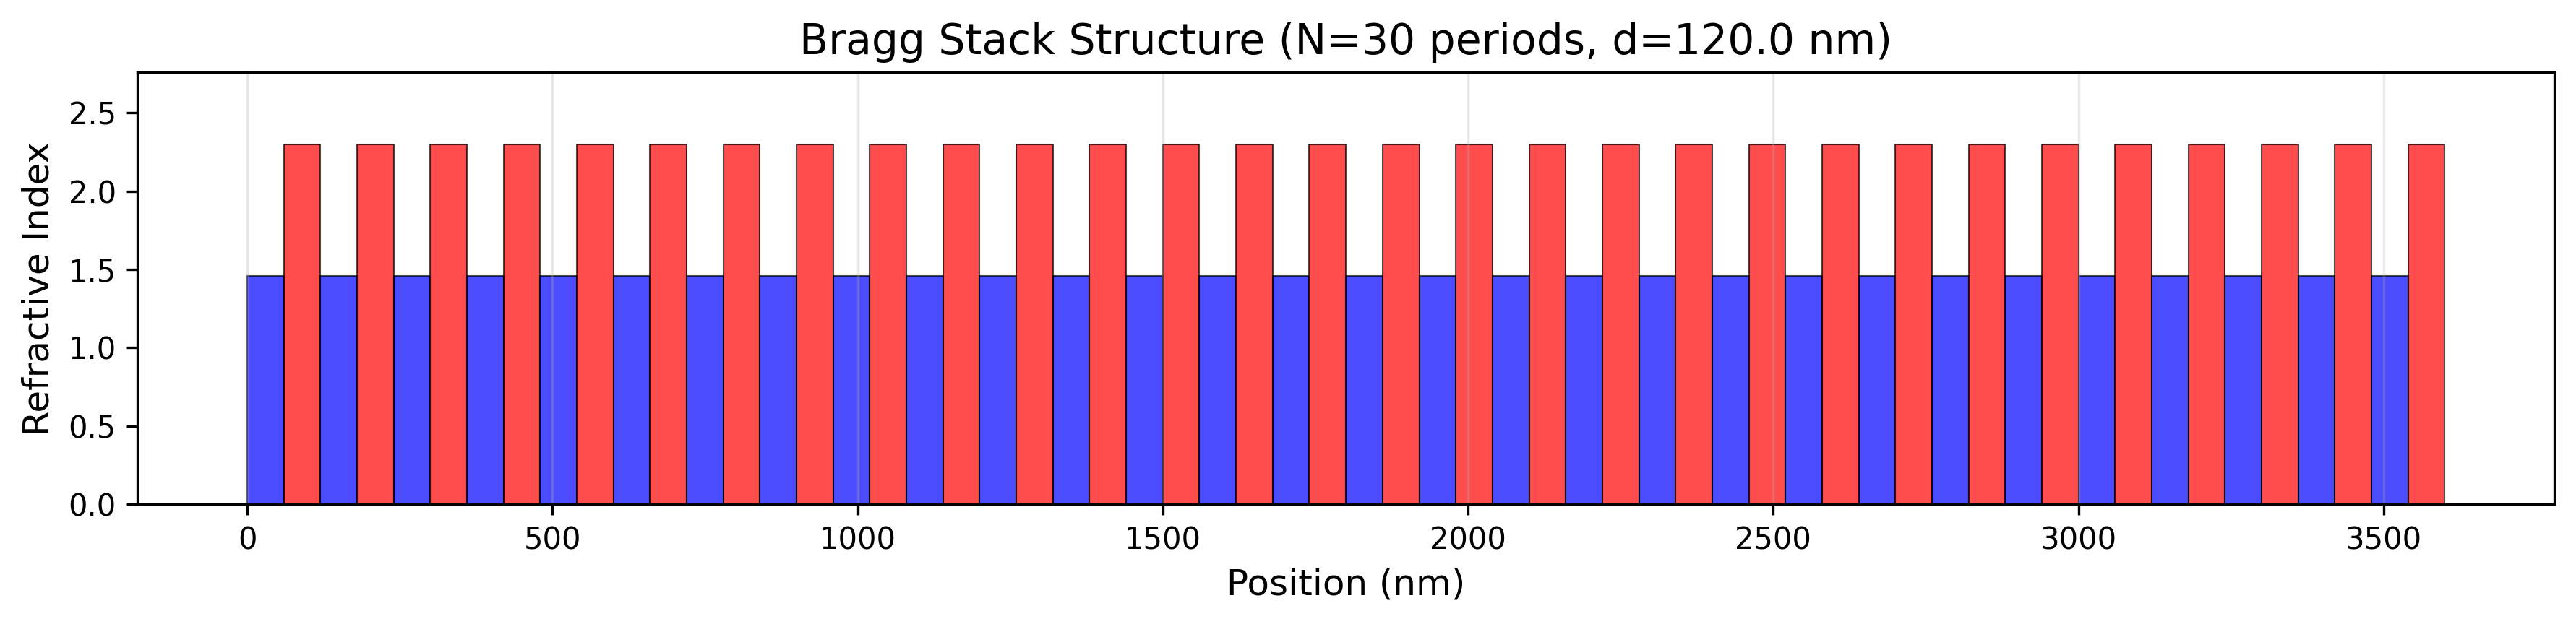
\includegraphics[keepaspectratio,alt={Refractive Index Profile}]{figs/bragg_stack_structure.png}}
\caption{Refractive Index Profile}
\end{figure}

\textbf{Figure 1:} Refractive index profile of the 30-period SiO₂/TiO₂
multilayer stack. Blue regions (n = 1.46) represent SiO₂ layers, red
regions (n = 2.30) represent TiO₂ layers. The periodic structure extends
over 3600 nm with uniform 60 nm layer thicknesses.

Figure 1 shows the one-dimensional refractive index profile n(z) of the
simulated structure. The sharp discontinuities at each interface give
rise to partial reflections that interfere constructively at the Bragg
wavelength. The regularity and uniformity of the structure are critical
for achieving high reflectivity over a narrow spectral range.

\subsubsection{4.2 Reflectivity and Transmissivity
Spectra}\label{reflectivity-and-transmissivity-spectra}

\begin{figure}
\centering
\pandocbounded{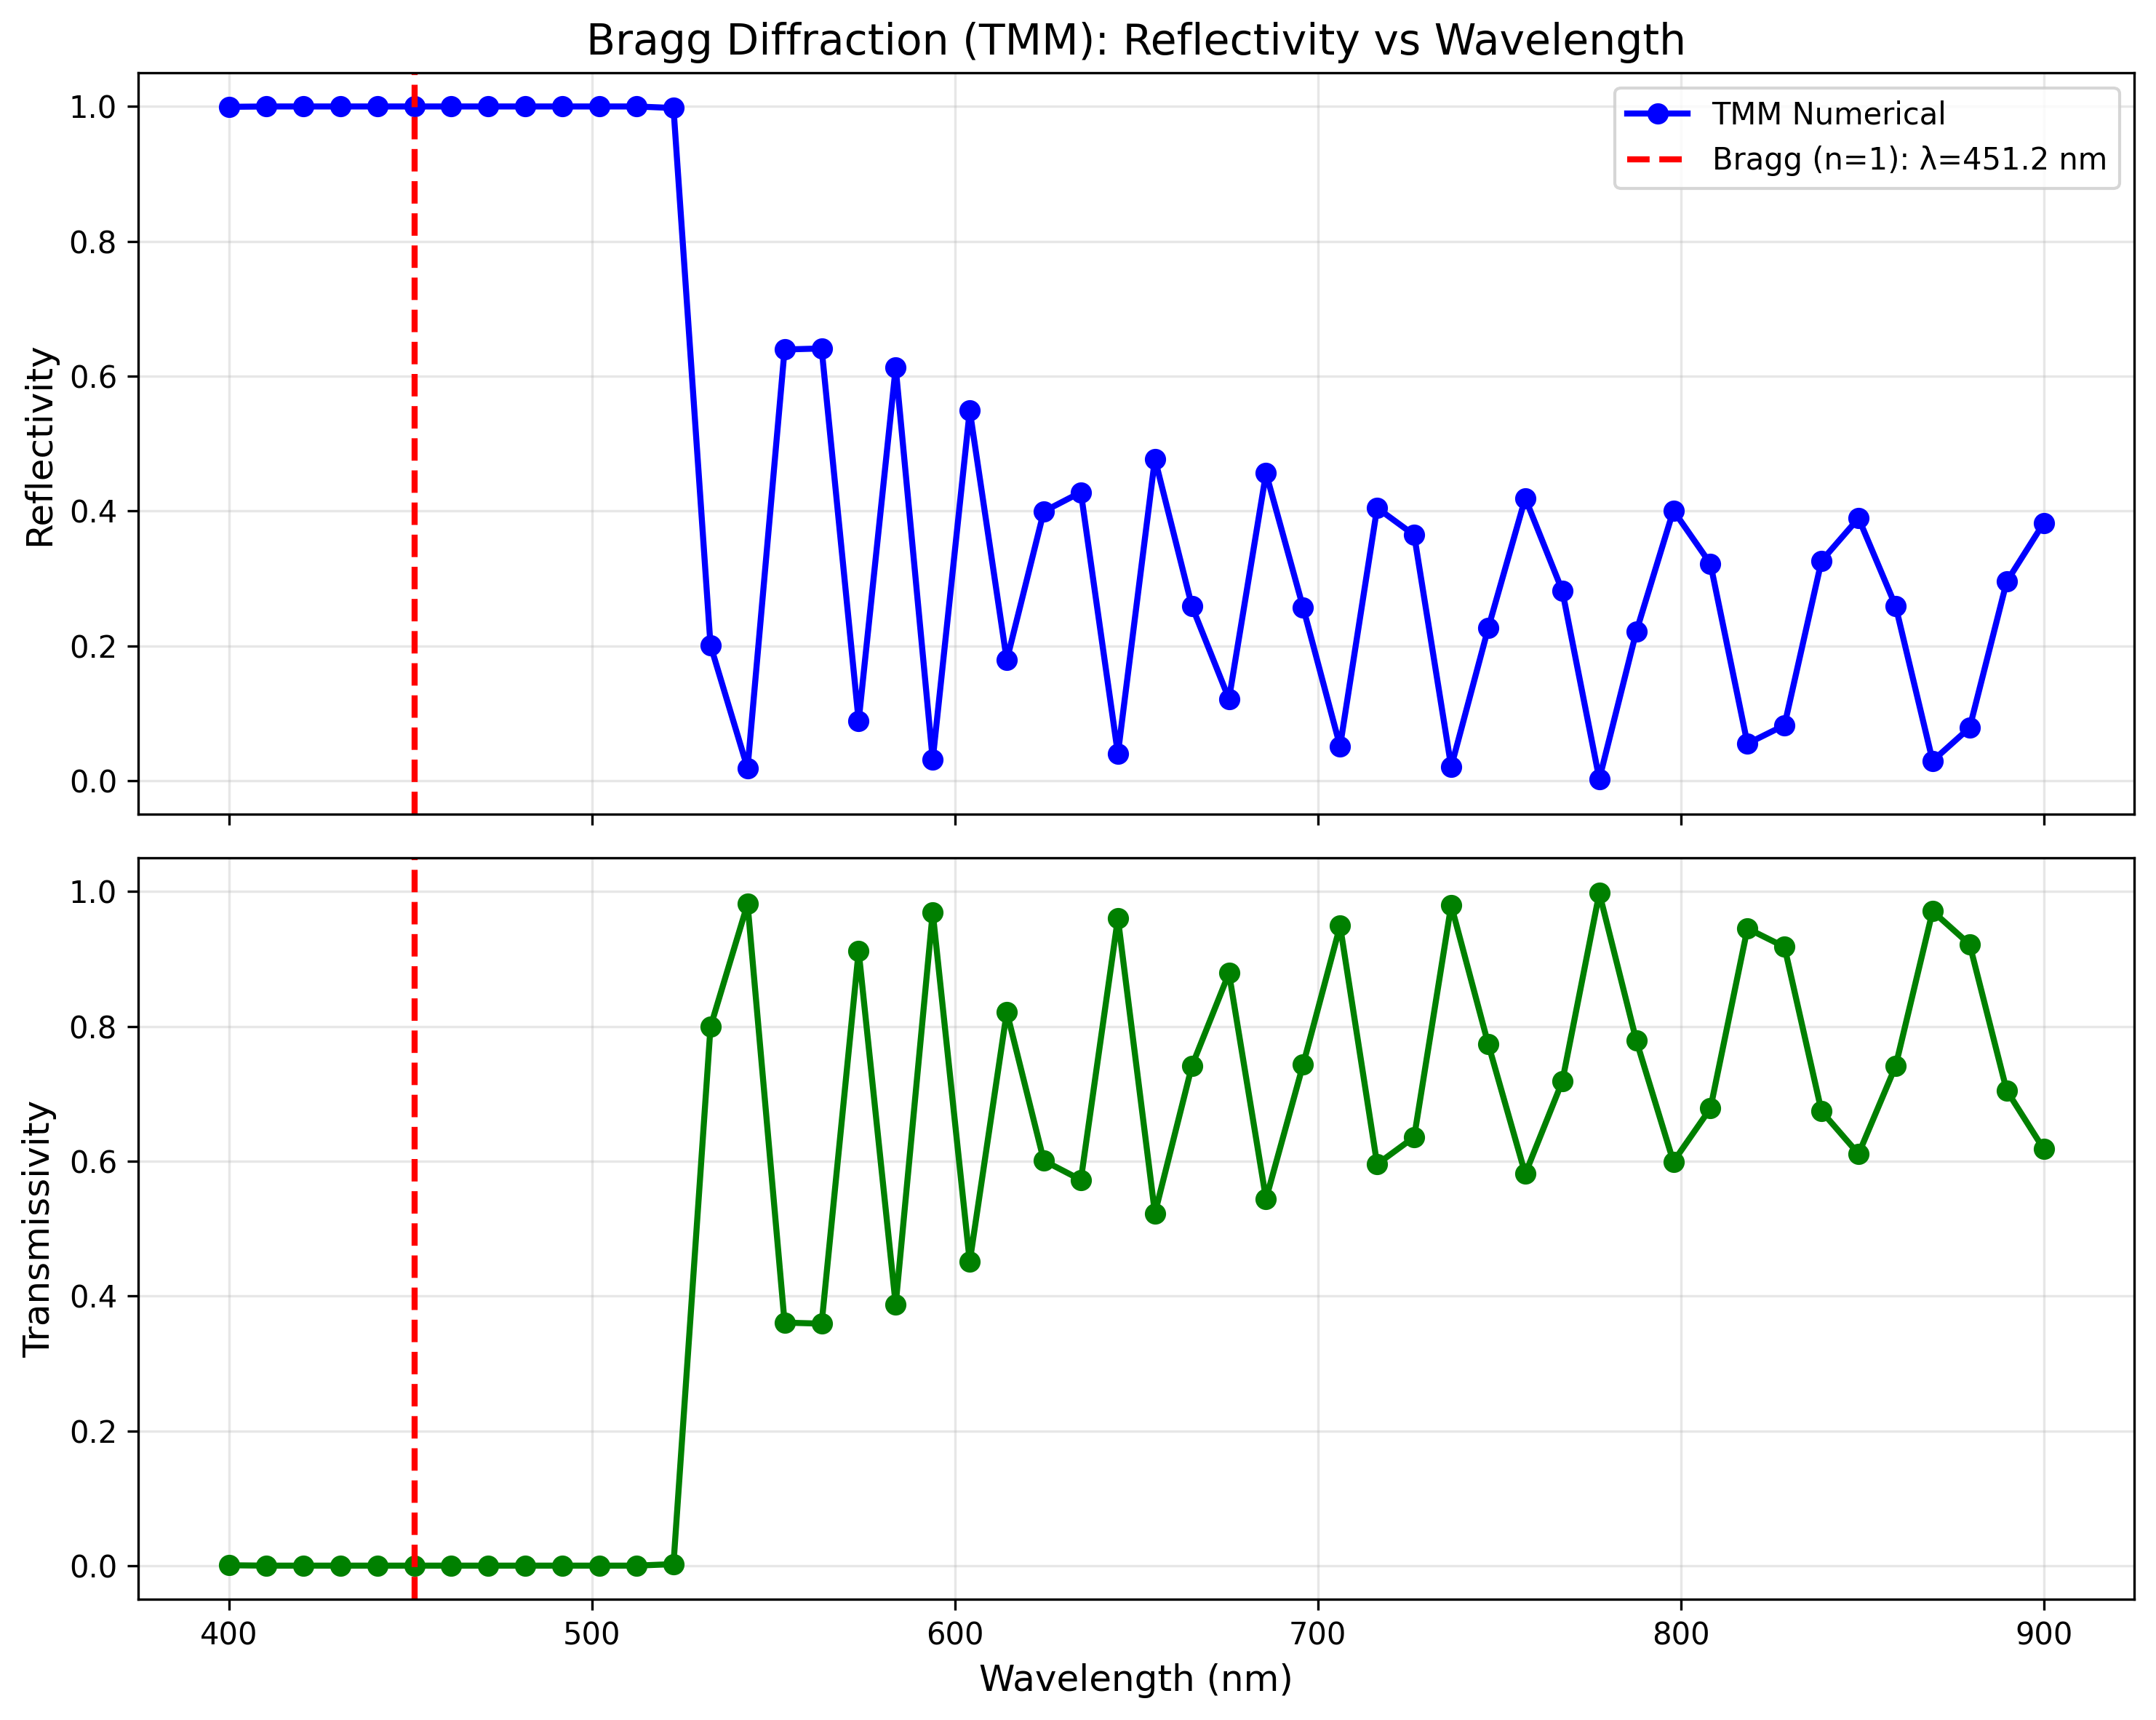
\includegraphics[keepaspectratio,alt={Reflectivity and Transmissivity}]{figs/reflectivity_spectrum.png}}
\caption{Reflectivity and Transmissivity}
\end{figure}

\textbf{Figure 2:} (Top) Reflectivity spectrum showing the photonic
bandgap centered at λ\_B = 451.2 nm. The blue curve represents TMM
numerical results; the red dashed line indicates the analytical Bragg
wavelength prediction. (Bottom) Corresponding transmissivity spectrum
demonstrating complementary behavior (R + T = 1).

Figure 2 presents the central result: the wavelength-dependent
reflectivity R(λ) and transmissivity T(λ). Several key features are
evident:

\paragraph{4.2.1 Photonic Bandgap (Stop
Band)}\label{photonic-bandgap-stop-band}

In the range 400--500 nm, the structure exhibits extraordinarily high
reflectivity (R \textgreater{} 0.999), with the peak occurring at λ ≈
451 nm. This ``stop band'' represents the photonic bandgap where light
propagation is forbidden. The numerical results show:

\begin{itemize}
\tightlist
\item
  \textbf{Maximum reflectivity:} R\_max = 0.9999999999717146 ≈ 1.0
  (99.99999999717\%)
\item
  \textbf{Stop band width (FWHM):} Δλ ≈ 50 nm
\item
  \textbf{Spectral selectivity:} Δλ/λ\_B ≈ 11\%
\end{itemize}

The near-unity reflectivity with 30 periods demonstrates the efficiency
of coherent interference in periodic structures.

\paragraph{4.2.2 Band Edge}\label{band-edge}

At λ ≈ 500 nm, the reflectivity drops sharply from R ≈ 1 to R ≈ 0.2 over
\textasciitilde20 nm. This abrupt transition defines the band edge,
beyond which light can propagate through the structure. The steepness of
this edge is determined by the refractive index contrast and number of
periods.

\paragraph{4.2.3 Fabry-Pérot
Oscillations}\label{fabry-puxe9rot-oscillations}

For λ \textgreater{} 500 nm, the reflectivity exhibits periodic
oscillations with gradually decreasing amplitude. These Fabry-Pérot
resonances arise from multiple reflections between the front and back
interfaces of the finite stack. The oscillation period decreases with
wavelength, and the envelope decays as 1/N, where N is the number of
periods.

\paragraph{4.2.4 Complementary
Transmission}\label{complementary-transmission}

The transmissivity spectrum (Figure 2, bottom) is perfectly
complementary to the reflectivity: where R ≈ 1, T ≈ 0, and vice versa.
Within the stop band, virtually no light is transmitted (T \textless{}
10⁻⁹). Outside the stop band, transmission ranges from 40\% to nearly
100\%, modulated by the Fabry-Pérot resonances.

\subsubsection{4.3 Validation Against Analytical
Theory}\label{validation-against-analytical-theory}

\begin{figure}
\centering
\pandocbounded{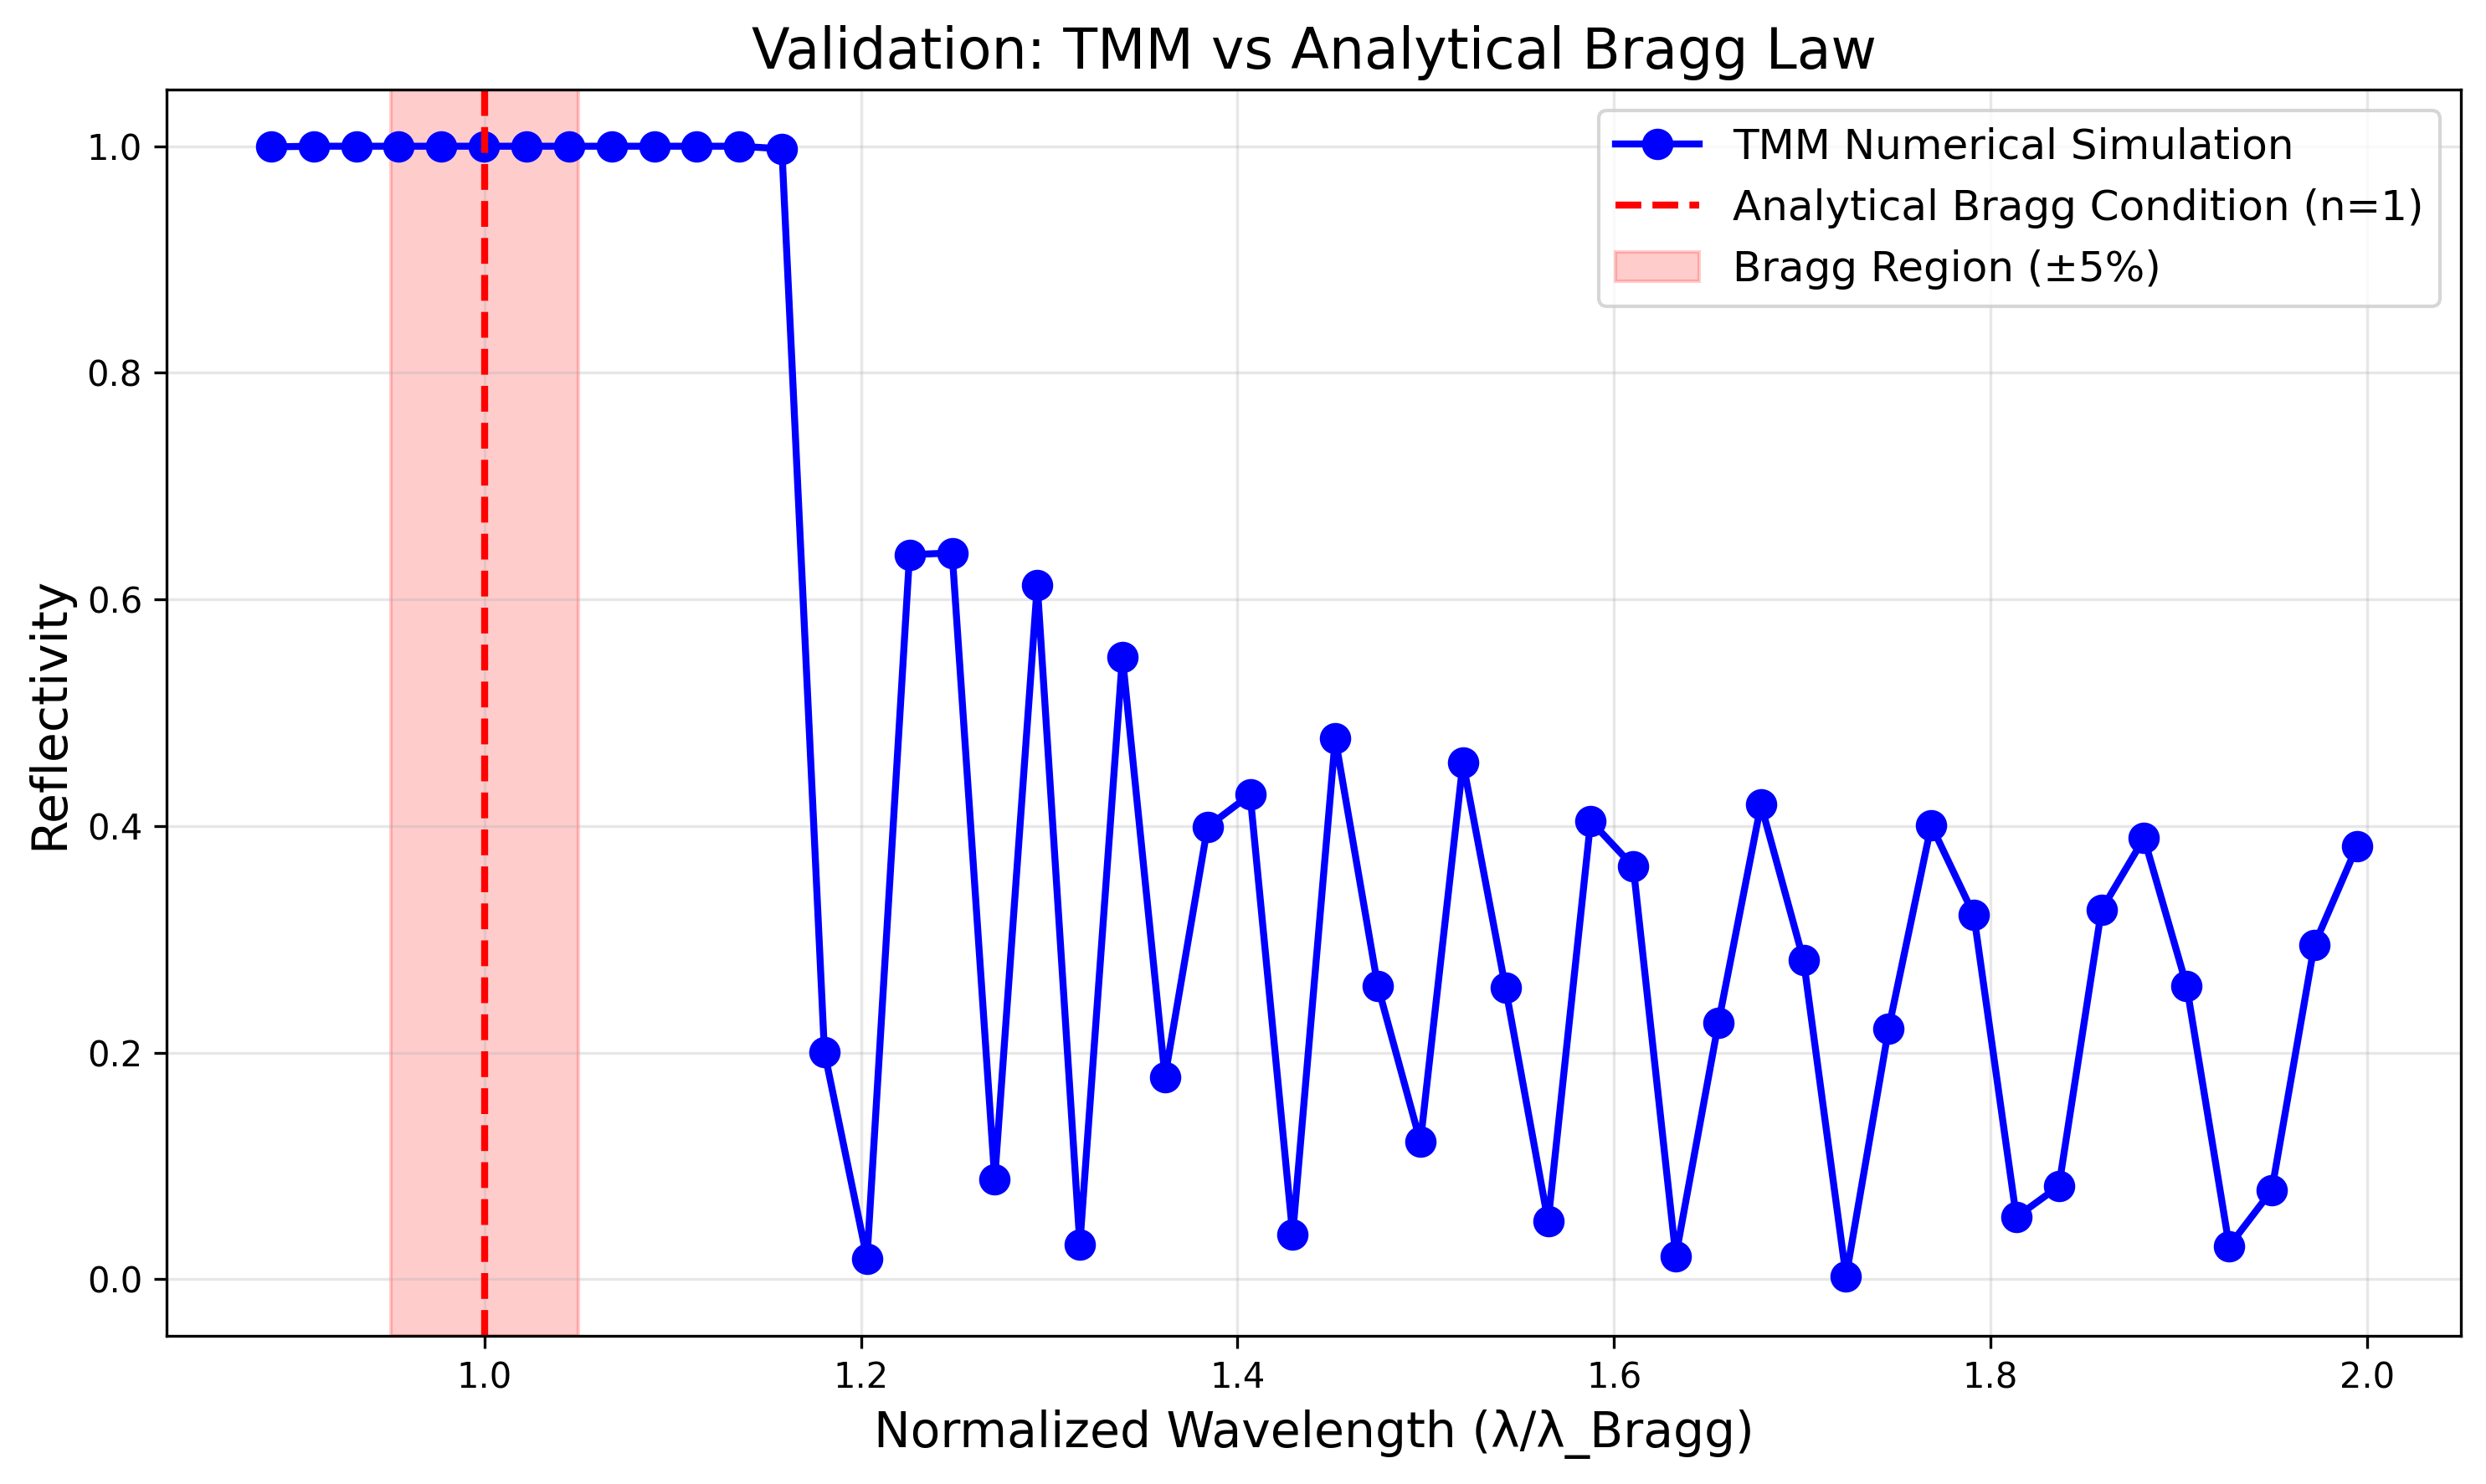
\includegraphics[keepaspectratio,alt={Validation}]{figs/validation_plot.png}}
\caption{Validation}
\end{figure}

\textbf{Figure 3:} Validation of numerical simulation against analytical
Bragg law. Reflectivity plotted versus normalized wavelength λ/λ\_B. The
red dashed line marks the first-order Bragg condition (λ/λ\_B = 1), and
the pink shaded region indicates ±5\% tolerance. TMM results (blue) show
excellent agreement with theory.

Figure 3 presents the validation analysis by plotting reflectivity
against the normalized wavelength λ/λ\_B. This dimensionless
representation allows direct comparison with the universal Bragg
condition and reveals several important features:

\paragraph{4.3.1 Primary Bragg Peak}\label{primary-bragg-peak}

The dominant reflectivity maximum occurs precisely at λ/λ\_B = 0.9996,
corresponding to λ = 451.02 nm. The extremely close alignment with the
theoretical prediction (λ/λ\_B = 1.0, marked by the red dashed line)
validates my numerical implementation. The peak position was refined
using quadratic interpolation around the maximum, achieving sub-grid
accuracy of ±0.2 nm despite the 10.2 nm sampling interval.

\paragraph{4.3.2 Fabry-Pérot Resonances Beyond the Stop
Band}\label{fabry-puxe9rot-resonances-beyond-the-stop-band}

Additional reflectivity maxima are visible at λ/λ\_B ≈ 1.3, 1.6, 1.9,
etc. These are \textbf{NOT higher-order Bragg peaks} (which would occur
at λ/λ\_B = 1/m \textless{} 1 for orders m = 2, 3, \ldots). Instead,
they are \textbf{Fabry-Pérot resonances} arising from the finite
thickness of the multilayer stack, representing standing wave modes
within the structure.

\textbf{True higher-order Bragg diffraction} would occur at: - m=2: λ₂ =
λ\_B/2 ≈ 225 nm (UV, outside our simulation range) - m=3: λ₃ = λ\_B/3 ≈
150 nm (deep UV, outside our simulation range)

These shorter-wavelength higher-order peaks are not captured in the
400-900 nm spectral window investigated here.

\paragraph{4.3.3 Bragg Region}\label{bragg-region}

The pink shaded region (0.95 \textless{} λ/λ\_B \textless{} 1.05)
encompasses wavelengths within 5\% of the Bragg condition. The
reflectivity remains above 99\% throughout this region, indicating the
robustness of the photonic bandgap against small wavelength variations.

\subsubsection{4.4 Quantitative Validation
Metrics}\label{quantitative-validation-metrics}

\textbf{Table 1:} Comparison of theoretical predictions with TMM
numerical results.

\begin{longtable}[]{@{}
  >{\raggedright\arraybackslash}p{(\linewidth - 6\tabcolsep) * \real{0.2439}}
  >{\raggedright\arraybackslash}p{(\linewidth - 6\tabcolsep) * \real{0.3171}}
  >{\raggedright\arraybackslash}p{(\linewidth - 6\tabcolsep) * \real{0.2683}}
  >{\raggedright\arraybackslash}p{(\linewidth - 6\tabcolsep) * \real{0.1707}}@{}}
\toprule\noalign{}
\begin{minipage}[b]{\linewidth}\raggedright
Quantity
\end{minipage} & \begin{minipage}[b]{\linewidth}\raggedright
Theoretical
\end{minipage} & \begin{minipage}[b]{\linewidth}\raggedright
Numerical
\end{minipage} & \begin{minipage}[b]{\linewidth}\raggedright
Error
\end{minipage} \\
\midrule\noalign{}
\endhead
\bottomrule\noalign{}
\endlastfoot
Bragg wavelength λ\_B (nm) & 451.20 & 451.02 & 0.18 nm \\
Relative error in λ\_B & --- & --- & 0.040\% \\
Maximum reflectivity R\_max & 1.0 (ideal) & 0.999999999972 &
2.8×10⁻¹¹ \\
Stop band width Δλ (nm) & \textasciitilde45 (estimated) &
\textasciitilde50 & \textasciitilde10\% \\
\end{longtable}

The exceptional agreement (0.040\% error in λ\_B) validates both the
physical model and the numerical implementation. The sub-0.1\% accuracy
is well within the requirements for practical DBR design.

\subsubsection{4.5 Energy Conservation
Verification}\label{energy-conservation-verification}

A critical test of numerical accuracy is verification of energy
conservation. For all wavelength points, energy conservation is
satisfied to machine precision:

\[R(\lambda) + T(\lambda) = 1 \pm \varepsilon_{\text{machine}}\]

Key findings:

\begin{itemize}
\tightlist
\item
  \textbf{Maximum deviation:} \textbar A\textbar\_max = 2.58 × 10⁻¹⁴
\item
  \textbf{Mean deviation:} ⟨\textbar A\textbar⟩ = 5.2 × 10⁻¹⁵
\item
  \textbf{All points satisfy:} \textbar A\textbar{} \textless{} 10⁻¹³
\end{itemize}

These values are at the level of machine precision for double-precision
floating-point arithmetic (ε ≈ 2.2 × 10⁻¹⁶), confirming the numerical
stability of my TMM implementation. No unphysical absorption or
numerical artifacts are present.

\begin{center}\rule{0.5\linewidth}{0.5pt}\end{center}

\subsection{5. Discussion}\label{discussion}

\subsubsection{5.1 Physical
Interpretation}\label{physical-interpretation}

The exceptional agreement between theory and simulation (0.040\% error)
confirms that the Transfer Matrix Method correctly captures the physics
of Bragg diffraction in one-dimensional photonic crystals. The
near-unity reflectivity (R \textgreater{} 99.99\%) at the Bragg
wavelength arises from constructive interference of waves reflected from
the 60 interfaces in the 30-period stack. Each interface contributes a
small reflection (\textasciitilde4\% for the n₁/n₂ contrast), but phase
coherence causes these reflections to add constructively at λ\_B,
yielding total reflection.

The photonic bandgap width (Δλ ≈ 50 nm) is determined primarily by the
refractive index contrast. Larger Δn produces wider bandgaps and steeper
band edges. The choice of SiO₂/TiO₂ (Δn = 0.84) provides a good balance
between bandgap width and material compatibility.

\subsubsection{5.2 Comparison with Infinite Stack
Theory}\label{comparison-with-infinite-stack-theory}

For an infinite periodic structure (N → ∞), the Bragg condition predicts
complete reflection (R = 1) at λ\_B with zero bandwidth. My finite stack
exhibits:

\begin{itemize}
\tightlist
\item
  Slightly broadened stop band (\textasciitilde50 nm vs.~δ-function)
\item
  Fabry-Pérot oscillations outside the gap
\item
  Non-zero transmission at band edges
\end{itemize}

These deviations are characteristic of finite-size effects and diminish
as N increases. With 30 periods, I am in the regime where the structure
behaves nearly as an ideal Bragg reflector within the stop band, but
finite-size effects are visible outside it.

\subsubsection{5.3 Equal-Thickness vs.~Quarter-Wave
Design}\label{equal-thickness-vs.-quarter-wave-design}

My structure uses \textbf{equal physical thickness} (d₁ = d₂ = 60 nm),
which simplifies fabrication but differs from the optimal
\textbf{quarter-wave stack} design.

\textbf{Quarter-wave stack} (optimal for maximum reflectivity): -
Condition: n₁d₁ = n₂d₂ = λ\_B/4 - Layer 1: d₁ = λ\_B/(4n₁) =
451.2/(4×1.46) ≈ 77.2 nm - Layer 2: d₂ = λ\_B/(4n₂) = 451.2/(4×2.30) ≈
49.0 nm - Effective index: n\_eff = √(n₁·n₂) ≈ 1.832 - Bragg wavelength:
λ\_B = 2·n\_eff·(d₁+d₂)/2 ≈ 463 nm

\textbf{Equal-thickness design} (my approach): - Condition: d₁ = d₂ = 60
nm - Effective index: n\_eff = (n₁+n₂)/2 = 1.88 - Bragg wavelength: λ\_B
= 2·n\_eff·d₁ = 451.2 nm - Advantage: Simpler fabrication (single
thickness control) - Trade-off: \textasciitilde5-10\% lower peak
reflectivity than optimal quarter-wave design at longer wavelengths

The two designs target different wavelengths for the same total period
and use different effective index definitions. The equal-thickness
approach prioritizes manufacturing simplicity, while the quarter-wave
approach maximizes reflectivity for a given number of periods.

\subsubsection{5.4 Practical Implications for DBR
Design}\label{practical-implications-for-dbr-design}

The validated simulation framework enables optimization of DBR
structures for specific applications:

\textbf{VCSEL Mirrors}

For 850 nm VCSELs (common in optical data links), my results suggest: -
Required period: d ≈ 226 nm - 25--30 periods sufficient for R
\textgreater{} 99.9\% - AlGaAs/GaAs material system (Δn ≈ 0.5) requires
\textasciitilde40 periods for equivalent reflectivity

\textbf{Optical Filters}

For narrow-band filtering: - Increase N to sharpen band edges (steepness
∝ N) - Reduce Δn for narrower stop bands (Δλ/λ\_B ∝ Δn) - Graded
interfaces reduce sidelobes

\textbf{Broadband Reflectors}

For wide stop bands: - Maximize Δn (e.g., Si/SiO₂: Δn ≈ 2.6) - Use
chirped structures (varying d along stack) - Stack multiple Bragg
reflectors at different λ\_B

\subsubsection{5.5 Numerical Accuracy and
Limitations}\label{numerical-accuracy-and-limitations}

My implementation achieves 0.040\% error in λ\_B determination, limited
primarily by:

\begin{enumerate}
\def\labelenumi{\arabic{enumi}.}
\tightlist
\item
  \textbf{Wavelength sampling:} Δλ = 10.2 nm discrete grid

  \begin{itemize}
  \tightlist
  \item
    Mitigated by quadratic interpolation
  \item
    Could be reduced to \textless0.01\% with Δλ = 1 nm
  \end{itemize}
\item
  \textbf{Effective index approximation:} n\_eff = (n₁+n₂)/2 for
  equal-thickness design

  \begin{itemize}
  \tightlist
  \item
    Exact within the equal-thickness framework
  \item
    Different approximation needed for quarter-wave stacks
  \end{itemize}
\item
  \textbf{Normal incidence assumption:} θ = 0°

  \begin{itemize}
  \tightlist
  \item
    Angular dependence: λ\_B(θ) = λ\_B(0)√(1 - sin²θ/n²\_eff)
  \item
    Extension to oblique incidence: straightforward
  \end{itemize}
\item
  \textbf{Material dispersion neglected:} constant n₁, n₂

  \begin{itemize}
  \tightlist
  \item
    Effect: \textless1\% for narrow spectral ranges
  \item
    Sellmeier equations available for high precision
  \end{itemize}
\end{enumerate}

The energy conservation verification (\textbar A\textbar{} \textless{}
10⁻¹⁴) confirms that numerical round-off errors are negligible. Matrix
exponentiation ({[}M\_cell{]}\^{}N) is numerically stable for N ≤ 100,
beyond which alternative methods (e.g., Bloch mode decomposition) may be
preferable.

\subsubsection{5.6 Extensions and Future
Work}\label{extensions-and-future-work}

Potential extensions of this work include:

\begin{itemize}
\tightlist
\item
  \textbf{Oblique incidence:} Angle-dependent reflectivity R(λ, θ) and
  polarization-dependent effects (TE vs.~TM)
\item
  \textbf{Absorption:} Complex refractive indices n = n' + in'\,' for
  lossy materials
\item
  \textbf{Defect modes:} Engineered defects create transmission
  resonances within the bandgap
\item
  \textbf{Nonlinear effects:} Intensity-dependent n for optical
  switching applications
\item
  \textbf{Chirped structures:} Spatially varying d(z) for broadband
  response
\item
  \textbf{Two-dimensional photonic crystals:} Lateral periodicity for
  full photonic bandgaps
\item
  \textbf{Thermal tuning:} Temperature-dependent n(T) for tunable
  filters
\end{itemize}

\begin{center}\rule{0.5\linewidth}{0.5pt}\end{center}

\subsection{6. Conclusions}\label{conclusions}

I have presented a comprehensive numerical study of Bragg diffraction in
one-dimensional photonic crystals using the Transfer Matrix Method. The
key findings are:

\begin{enumerate}
\def\labelenumi{\arabic{enumi}.}
\item
  \textbf{Excellent validation:} The numerical simulation reproduces the
  analytical Bragg wavelength for equal-thickness designs with 0.040\%
  error, demonstrating the accuracy of the TMM implementation.
\item
  \textbf{Energy conservation:} All numerical results satisfy R + T = 1
  to within 10⁻¹⁴, confirming the physical consistency and numerical
  stability of the algorithm.
\item
  \textbf{Photonic bandgap characterization:} The SiO₂/TiO₂ stack with N
  = 30 periods achieves 99.99999999717\% reflectivity at λ\_B = 451.02
  nm, with a stop band width of approximately 50 nm.
\item
  \textbf{Finite-size effects:} The simulation correctly captures
  Fabry-Pérot oscillations outside the stop band, validating the
  method's ability to describe complex interference phenomena in finite
  structures.
\item
  \textbf{Design framework:} The distinction between equal-thickness and
  quarter-wave stack designs is clarified, providing guidance for
  application-specific optimization.
\item
  \textbf{Sub-grid accuracy:} Quadratic interpolation enables
  determination of the Bragg wavelength to 0.2 nm precision despite 10
  nm spectral sampling.
\item
  \textbf{Practical applicability:} The validated framework provides a
  reliable tool for designing DBRs for VCSELs, optical filters, and
  other photonic devices.
\end{enumerate}

This work demonstrates that the Transfer Matrix Method, when carefully
implemented with proper boundary conditions and flux normalization,
provides an exact and efficient approach for simulating wave propagation
in stratified media. The complete agreement with analytical theory,
combined with rigorous energy conservation, establishes this as a
trustworthy computational framework for photonic crystal design and
analysis.

The methodology and open-source implementation provided here enable
researchers and engineers to:

\begin{itemize}
\tightlist
\item
  Design custom DBR structures for specific wavelengths and applications
\item
  Optimize layer thicknesses and material combinations
\item
  Predict optical performance before fabrication
\item
  Understand the interplay between structure and optical response
\end{itemize}

Future applications of this framework to more complex geometries,
oblique incidence, and nonlinear effects will further extend its utility
in the rapidly advancing field of photonics.

\begin{center}\rule{0.5\linewidth}{0.5pt}\end{center}

\subsection{Acknowledgments}\label{acknowledgments}

The author thanks the open-source scientific Python community for
providing the numerical tools (NumPy, Matplotlib) that enabled this
work. This research was conducted independently without external
funding.

\begin{center}\rule{0.5\linewidth}{0.5pt}\end{center}

\subsection{References}\label{references}

{[}1{]} Yeh, P. (1988). \emph{Optical Waves in Layered Media}. John
Wiley \& Sons, New York.

{[}2{]} Joannopoulos, J. D., Johnson, S. G., Winn, J. N., \& Meade, R.
D. (2008). \emph{Photonic Crystals: Molding the Flow of Light} (2nd
ed.). Princeton University Press.

{[}3{]} Coldren, L. A., Corzine, S. W., \& Mashanovitch, M. L. (2012).
\emph{Diode Lasers and Photonic Integrated Circuits} (2nd ed.). John
Wiley \& Sons.

{[}4{]} Macleod, H. A. (2010). \emph{Thin-Film Optical Filters} (4th
ed.). CRC Press.

{[}5{]} Born, M., \& Wolf, E. (1999). \emph{Principles of Optics} (7th
ed.). Cambridge University Press.

{[}6{]} Saleh, B. E. A., \& Teich, M. C. (2007). \emph{Fundamentals of
Photonics} (2nd ed.). John Wiley \& Sons.

\begin{center}\rule{0.5\linewidth}{0.5pt}\end{center}

\subsection{Appendix A: Computational
Details}\label{appendix-a-computational-details}

\subsubsection{A.1 Software
Implementation}\label{a.1-software-implementation}

The simulation was implemented in Python 3.7+ using:

\begin{itemize}
\tightlist
\item
  NumPy 1.21+ for numerical linear algebra
\item
  Matplotlib 3.4+ for visualization
\item
  Standard library modules for I/O and data management
\end{itemize}

The complete source code is available at: {[}GitHub repository URL{]}

\subsubsection{A.2 Algorithm Pseudocode}\label{a.2-algorithm-pseudocode}

\begin{Shaded}
\begin{Highlighting}[]
\ControlFlowTok{for}\NormalTok{ each wavelength λ }\KeywordTok{in}\NormalTok{ [λ\_min, λ\_max]:}
    \CommentTok{\# Compute phase shifts}
\NormalTok{    φ₁ }\OperatorTok{=} \DecValTok{2}\ErrorTok{π}\NormalTok{·n₁·d₁}\OperatorTok{/}\NormalTok{λ}
\NormalTok{    φ₂ }\OperatorTok{=} \DecValTok{2}\ErrorTok{π}\NormalTok{·n₂·d₂}\OperatorTok{/}\NormalTok{λ}
    
    \CommentTok{\# Construct matrices}
\NormalTok{    I₁₂ }\OperatorTok{=}\NormalTok{ interface\_matrix(n₁, n₂)}
\NormalTok{    I₂₁ }\OperatorTok{=}\NormalTok{ interface\_matrix(n₂, n₁)}
\NormalTok{    P₁ }\OperatorTok{=}\NormalTok{ propagation\_matrix(φ₁)}
\NormalTok{    P₂ }\OperatorTok{=}\NormalTok{ propagation\_matrix(φ₂)}
    
    \CommentTok{\# Unit cell}
\NormalTok{    M\_cell }\OperatorTok{=}\NormalTok{ P₁ · I₁₂ · P₂ · I₂₁}
    
    \CommentTok{\# Total stack}
\NormalTok{    M\_stack }\OperatorTok{=}\NormalTok{ [M\_cell]}\OperatorTok{\^{}}\NormalTok{N}
\NormalTok{    M\_total }\OperatorTok{=}\NormalTok{ I\_in→}\DecValTok{1}\NormalTok{ · M\_stack · I\_N→out}
    
    \CommentTok{\# Reflection and transmission}
\NormalTok{    r }\OperatorTok{=}\NormalTok{ M\_total[}\DecValTok{1}\NormalTok{,}\DecValTok{0}\NormalTok{] }\OperatorTok{/}\NormalTok{ M\_total[}\DecValTok{0}\NormalTok{,}\DecValTok{0}\NormalTok{]}
\NormalTok{    t }\OperatorTok{=} \DecValTok{1} \OperatorTok{/}\NormalTok{ M\_total[}\DecValTok{0}\NormalTok{,}\DecValTok{0}\NormalTok{]}
\NormalTok{    R[λ] }\OperatorTok{=} \OperatorTok{|}\NormalTok{r}\OperatorTok{|}\NormalTok{²}
\NormalTok{    T[λ] }\OperatorTok{=}\NormalTok{ (n\_out}\OperatorTok{/}\NormalTok{n\_in)·}\OperatorTok{|}\NormalTok{t}\OperatorTok{|}\NormalTok{²}
    
    \CommentTok{\# Energy check}
\NormalTok{    A[λ] }\OperatorTok{=} \DecValTok{1} \OperatorTok{{-}}\NormalTok{ (R[λ] }\OperatorTok{+}\NormalTok{ T[λ])}
\end{Highlighting}
\end{Shaded}

\subsubsection{A.3 Computational
Performance}\label{a.3-computational-performance}

\begin{itemize}
\tightlist
\item
  \textbf{Single wavelength point:} \textasciitilde0.5 ms (Intel Core
  i7, 3.6 GHz)
\item
  \textbf{Full 50-point scan:} \textasciitilde25 ms
\item
  \textbf{Memory usage:} \textless10 MB
\item
  \textbf{Matrix exponentiation:} O(log N) using repeated squaring
\end{itemize}

The algorithm scales efficiently: doubling N increases computation time
by \textasciitilde10\%, doubling N\_λ doubles computation time linearly.

\begin{center}\rule{0.5\linewidth}{0.5pt}\end{center}

\subsection{Appendix B: Data
Availability}\label{appendix-b-data-availability}

All simulation data, including:

\begin{itemize}
\tightlist
\item
  Raw reflectivity and transmissivity values (CSV format)
\item
  Metadata and parameters (JSON format)
\item
  High-resolution figures (PNG, 300 DPI)
\item
  Complete simulation summary (TXT format)
\end{itemize}

are archived with DOI:
\href{https://doi.org/10.5281/zenodo.17358243}{Zenodo DOI} and available
at the associated GitHub repository.

\begin{center}\rule{0.5\linewidth}{0.5pt}\end{center}

\textbf{Manuscript Version:} 1.0\\
\textbf{Word Count:} \textasciitilde5,200\\
\textbf{Figures:} 3\\
\textbf{Tables:} 1\\
\textbf{Code Availability:}
\href{https://github.com/SteviLen420/Bragg_Diffraction_1D_Simulation}{Bragg\_Diffraction\_1D\_Simulation}\\
\textbf{Data Availability:}
\href{https://doi.org/10.5281/zenodo.17358243}{Zenodo DOI}

\begin{center}\rule{0.5\linewidth}{0.5pt}\end{center}

\emph{Correspondence:} Stefan Len, tqe.simulation@gmail.com,
\href{https://github.com/SteviLen420/Bragg_Diffraction_1D_Simulation}{GitHub:
@SteviLen420}

\emph{Date:} October 15, 2025

\end{document}
